% Fakesection 序言之前

\RequirePackage[l2tabu, orthodox]{nag}
\RequirePackage{ifxetex}
\RequireXeTeX

\documentclass{article}

%颜色
\usepackage{xcolor}

%长度
\usepackage{printlen}
\uselengthunit{mm}

%图形
\usepackage{pifont}
\usepackage{ean13isbn}
\usepackage{qrcode}
\usepackage{pdfpages}
\usepackage{overpic}
\usepackage{graphicx}
\graphicspath{{./src/}}
\usepackage{media9}
\usepackage{wallpaper}
\usepackage{wrapfig}

%表格
\usepackage{tabu}
\usepackage{longtable}
\usepackage{booktabs}
\usepackage{diagbox}
\usepackage{multicol}
\usepackage{multirow}
\usepackage{makecell}
\usepackage{fancybox}
\usepackage{colortbl}
\usepackage{tcolorbox}
\tcbuselibrary{skins}
\tcbuselibrary{breakable}
\tcbuselibrary{theorems}
\tcbuselibrary{listings}
\tcbuselibrary{xparse}
\tcbuselibrary{minted}% 用minted排版代码
\usepackage{fvextra}
\usepackage{csvsimple}
\usepackage{boxedminipage2e}

%公式
\usepackage{amsmath}
\usepackage{amsthm}
\usepackage{amsfonts}
\usepackage{amssymb}
\usepackage{amsbsy}
\usepackage{amsopn}
\usepackage{amstext}
\usepackage{mathrsfs}
\usepackage{bm}
\usepackage{textcomp}
\usepackage{latexsym}
\usepackage{exscale}
\usepackage{relsize}
%\usepackage{xymtex}
\usepackage{physics}
\usepackage{siunitx}
\usepackage{hologo}
\usepackage{cases}

%文字
\usepackage{csquotes}
\usepackage{microtype}
\usepackage[heading=true]{ctex}
\setCJKfamilyfont{zhsong}[AutoFakeBold = {2.17}]{SimSun}
\renewcommand*{\songti}{\CJKfamily{zhsong}}

%正文
\usepackage{fancyhdr}
\usepackage{geometry}
\usepackage{lastpage}
\usepackage{indentfirst}
\usepackage{setspace}
\renewcommand\arraystretch{1}

%非正文
\usepackage{makeidx}
\makeindex
\usepackage{epigraph}
\usepackage{varwidth}
\usepackage{exercise}
\usepackage{tasks}
\renewcommand{\ExerciseName}{问题}
\renewcommand{\AnswerName}{回答}
\renewcommand{\listexercisename}{问题}

%参考文献
\usepackage{morewrites}
\renewcommand{\thefootnote}{\fnsymbol{footnote}}
\usepackage[resetlabels]{multibib}

%标题
\usepackage{caption}
\usepackage{subcaption}
\newcounter{sub}

%其它
\usepackage{atbegshi}
\usepackage{lipsum}

\csname
endofdump
\endcsname

%代码
\usepackage{minted}
\usepackage{boxie}
\makeatletter
\xdefinecolor{tcbcol@back}{rgb}{0,0,0}
\makeatother

%链接%与beamer 冲突
\usepackage[
colorlinks = true,
linkcolor = gray,
citecolor = gray,
backref=page
]{hyperref}

%枚举%与beamer 干涉
\usepackage{enumitem}
\setlist[enumerate, 2]{
	fullwidth,
	label = \alph*.,
	font = \textup,
	itemindent=2em
}

%标题%与beamer 冲突
\usepackage{titlesec}
%\titleformat{\chapter}{\centering\Huge\bfseries}{实验\chinese{chapter}~}{0pt}{}
\titleformat{\section}{\centering\LARGE\bfseries}{\S\ifthenelse{\value{section}=0}{}{\thesection}~}{0pt}{}
%\titleformat{\subsection}{\Large}{\chinese{subsection}、~}{0pt}{}
%\titleformat{\subsubsection}{\large}{\arabic{subsubsection}.~}{0pt}{}

\begin{document}

% Fakesection 承诺书

%页眉页脚%与book冲突
\pagestyle{fancy}
%\renewcommand{\headrulewidth}{0pt}
\lhead{\zihao{4}赛区评阅编号(由赛区组委会填写):}
\chead{}
\rhead{}
\lfoot{}
\cfoot{}
\rfoot{}

\newcommand{\NumberCUMCMMathModeling}{201910047067}
\newcommand{\NumberProblem}{A}
\newcommand{\MemberOne}{吴振宇}
\newcommand{\MemberTwo}{尹卓异}
\newcommand{\MemberThree}{张文奇}
\newcommand{\MemberTeacher}{谢建春}
\newcommand{\MembersUniversity}{南京理工大学}
\newcommand{\Year}{2019}
\newcommand{\Month}{9}
\newcommand{\Day}{14}

\newif\ifCUMCMMathModeling\CUMCMMathModelingtrue

\ifnum\strcmp{\jobname}{\NumberCUMCMMathModeling}=0
	\CUMCMMathModelingfalse
\fi

% Fakesubsection 高教社杯全国大学生数学建模竞赛

\ifCUMCMMathModeling

	\newgeometry{left=2.5cm,right=2.5cm,top=3cm}

	\begin{center}
		\textbf{\zihao{3}\Year 年高教社杯全国大学生数学建模竞赛}

		\vspace{2em}

		\textbf{\zihao{3}承~诺~书}

		\vspace{1em}
	\end{center}

	\begin{spacing}{1.5}

		{\zihao{-4}

			我们仔细阅读了《全国大学生数学建模竞赛章程》和《全国大学生数学建模竞赛参赛规则》(2019年修订稿,以下简称为“竞赛章程和参赛规则”,可从全国大学生数学建模竞赛网站下载)。

			我们完全清楚,在竞赛开始后参赛队员不能以任何方式,包括电话、电子邮件、“贴吧”、QQ群、微信群等,与队外的任何人(包括指导教师)交流、讨论与赛题有关的问题;无论主动参与讨论还是被动接收讨论信息都是严重违反竞赛纪律的行为。

			我们完全清楚,抄袭别人的成果是违反竞赛章程和参赛规则的行为;如果引用别人的成果或资料(包括网上资料),必须按照规定的参考文献的表述方式列出,并在正文引用处予以标注。

			\textbf{我们以中国大学生名誉和诚信郑重承诺,严格遵守竞赛章程和参赛规则,以保证竞赛的公正、公平性。如有违反竞赛章程和参赛规则的行为,我们将受到严肃处理。}

			我们授权全国大学生数学建模竞赛组委会,可将我们的论文以任何形式进行公开展示(包括进行网上公示,在书籍、期刊和其他媒体进行正式或非正式发表等)。

			我们参赛选择的题号是(从A/B/C/D/E中选择一项填写):\underline{\makebox[12\ccwd][c]{\NumberProblem}}

			我们的报名参赛报名号为(12位数字全国统一编号):\underline{\makebox[12\ccwd][c]{\NumberCUMCMMathModeling}}

			所属学校(完整的学校全称,不含院系名):\underline{\makebox[20\ccwd][c]{\MembersUniversity}}

			参赛队员(打印并签名):1.\underline{\makebox[12\ccwd][c]{\MemberOne}}

			\makebox[11.5\ccwd][c]{}2.\underline{\makebox[12\ccwd][c]{\MemberTwo}}

			\makebox[11.5\ccwd][c]{}3.\underline{\makebox[12\ccwd][c]{\MemberThree}}

			指导教师或指导教师组负责人  (打印并签名):\underline{\makebox[12\ccwd][c]{\MemberTeacher}}

			\kaishu{(指导教师签名意味着对参赛队的行为和论文的真实性负责)}

			\begin{flushright}
				\songti
				日期:\underline{\makebox[4\ccwd][c]{\Year}}年\underline{\makebox[2\ccwd][c]{\Month}}月\underline{\makebox[2\ccwd][c]{\Day}}日
			\end{flushright}

			\textbf{\kaishu{(请勿改动此页内容和格式。此承诺书打印签名后作为纸质论文的封面,注意电子版论文中不得出现此页。以上内容请仔细核对,如填写错误,论文可能被取消评奖资格。)}}
		}

	\end{spacing}

	\newpage

	% Fakesubsection 高教社杯全国大学生数学建模竞赛编号专用页

	\begin{center}
		\textbf{\zihao{-3}\Year 年高教社杯全国大学生数学建模竞赛}

		\vspace{2em}

		\textbf{\zihao{3}编~号~专~用~页}

		\vspace{2em}
	\end{center}

	{\zihao{4}

		赛区评阅记录(可供赛区评阅时使用):

		\begin{tabu}to\linewidth{@{}|X[c,.3]|X[c]|X[c]|X[c]|X[c]|X[c]|X[c]|@{}}
			\hline
			 评阅人  &  &  &  &  &  &  \\ \hline
			 备注  &  &  &  &  &  &  \\ \hline
		\end{tabu}

		\vspace{5em}

		送全国评阅统一编号(赛区组委会填写):

		\vspace{10em}

		全国评阅随机编号(全国组委会填写):
	}

	\vspace{5em}

	\textbf{\kaishu{\zihao{-4}(请勿改动此页内容和格式。此承诺书打印签名后作为纸质论文的封面,注意电子版论文中不得出现此页。以上内容请仔细核对,如填写错误,论文可能被取消评奖资格。)}}

	\restoregeometry
	\setcounter{page}{1}

\fi

%页眉页脚%与book冲突
\pagestyle{fancy}
%\renewcommand{\headrulewidth}{0pt}
\lhead{\small{\leftmark}}
\chead{\small{\rightmark}}
\rhead{\small{第\thepage 页~共~\pageref{LastPage}~页}}
\lfoot{}
\cfoot{}
\rfoot{}

% Fakesection 摘要

\title{\textbf{}}
\author{}
\date{}
\maketitle

\renewcommand{\abstractname}{\Large 摘要}
\begin{abstract}
	本文对喷油过程进行分析,先通过龙格库塔法求出压强和密度的关系,并比较了其与简单的单步法的及精度差异。后建立了模型进行求解,并在二三问中通过启发式算法,在较短时间内求出了较为信服的解。
\end{abstract}

\textbf{关键词:龙格库塔法;单步法;遗传算法。}

\newpage

% Fakesection 目录

\pagenumbering{roman}

\tableofcontents
\listoffigures
\listoftables
\listofexercises

\newpage

\setcounter{section}{-1}

\pagenumbering{arabic}

\section{引言}%
\label{sec:引言}

\subsection{背景}%
\label{sub:背景}
党的十六大报告指出,“坚持以信息化带动工业化,以工业化促进信息化,走出一条科技含量高、经济效益好、资源消耗低、环境污染少、人力资源优势得到充分发挥的新型工业化路子。”新型工业化道路建设成为国家层面的核心战略。在这一背景下,提高工业化设备工作效率成为新型工业化建设的关键一环。

其中,燃油发动机,作为不少工业设备(例如汽车)中的核心装置,成为不少科研院所与工业企业关注的焦点。燃油发动机的工作基础是燃油进入和喷出高压油管,这一过程中燃油进入和喷出的间歇性工作过程会导致高压油管内压力变化,使喷出的燃油量出现偏差,影响发动机工作效率。因此,高压油管的压力控制是解决效率问题的关键。\cite{2011柴油机高压共轨分段喷射压力控制系统}


\subsection{问题重述}%
\label{sub:问题重述}
\subsubsection{问题1}
\begin{enumerate}
	\item \textbf{已知条件:}
		\begin{enumerate}
			\item 高压油管尺寸:内腔长度500mm,内直径10mm。
			\item 供油特性:供油入口小孔直径1.4mm,单向阀(控制供油时间)每打开一次后要关闭10ms。
			\item 喷油特性:喷油器每秒工作10次,每次喷油时间2.4ms,喷油速率由曲线给出。
			\item 压力特性:入口处压力恒为160MPa,高压油管内初始压力为100MPa。
		\end{enumerate}

	\item \textbf{目标任务:}
		\begin{enumerate}
			\item 如果要使高压油管内的压力尽可能稳定在100 MPa左右,求解单向阀每次开启的时长。
			\item 如果要使高压油管内的压力分别经过约2s、5s和10s的调整后稳定在150 MPa,求解单向阀开启的时长。
		\end{enumerate}
\end{enumerate}


\subsubsection{问题2}
\begin{enumerate}
	\item \textbf{已知条件:}
		\begin{enumerate}
			\item 供油特性:凸轮(驱动柱塞上下运动)边缘曲线与角度的关系由表格给出,燃油进入高压油管的条件是柱塞腔内的压力大于高压油管内的压力,柱塞腔直径5mm,柱塞运动到上止点时柱塞腔残余容积为$20\text{mm}^3$,柱塞运动到下止点时低压燃油充满柱塞腔且压力为0.5MPa。
			\item 喷油特性:针阀直径2.5mm,密封座是半角为9的圆锥,最下端喷孔直径1.4mm。针阀升程大于0时开启,燃油向喷孔流动并有喷孔喷出。一个喷油周期内针阀升程与时间的关系由表格给出。
		\end{enumerate}

	\item \textbf{目标任务:}

		采用问题1的喷油器工作次数、高压油管尺寸和初始压力,若要使得高压油管内的压力尽量稳定在100 MPa左右,确定凸轮角速度。
\end{enumerate}


\subsubsection{问题3}
\begin{enumerate}
	\item \textbf{供油端:}在供油入口下侧旁边安装一个出口直径为1.4mm的单向减压阀,其被打开后可以使高压油管内的燃油在压力下回流到外部低压油路中,从而减小高压油管内燃油的压力。据此调整喷油和供油策略。
	\item \textbf{喷油端:}在原喷油嘴旁边增加一个喷油规律相同的喷油嘴。设计高压油泵和减压阀的控制方案。
\end{enumerate}

\subsection{假设}%
\label{sub:假设}
\begin{enumerate}
	\item 凸轮匀速转动;
	\item 减速阀周期变化,在每个周期只打开关闭一次。
\end{enumerate}

\subsection{标记}%
\label{sub:标记}

\begin{table}[htpb]
	\centering
	\caption{标记}
	\label{tab:标记}
	\csvautobooktabular{src/notation.csv}
\end{table}

\section{模型准备与建立}
\subsection{压力-密度关系的构建}
压力$ p $与密度$ \rho $的关系符合式\ref{eq:rou}。其中弹性模量$ E $是随压力$ p $变化的单值函数。求解此微分方程可以得到压力$ p $与密度$ \rho $的关系。

\begin{align}
	\dv{}{\rho}p = \frac{E(p)}{\rho}
	\label{eq:rou}
\end{align}

将$E$与$\rho$视作$P$的函数,即$E(P)$和$\rho(P)$,则上式可化为:

\begin{equation}
	\rho'(P)=\frac{\rho(P)}{E(P)}
\end{equation}

题目给出了压力$P$与弹性模量$E$的配对关系,经过简单分析可知,所给数据为离散点,且有着明显的正相关关系。

为了提升数值计算的精度,本文首先采用最小二乘法对数据进行拟合,得到高度近似的拟合方程。最小二乘法的公式如下式所示:
\begin{equation}
	\left\{
		\begin{array}{ll}
			a_0 \Sigma \omega_i + a_1 \Sigma \omega_i x_i + \ldots +  a_n \Sigma \omega_i x_i^n =\Sigma \omega_i f(x_i) \\
			a_0 \Sigma \omega_i x_i + a_1 \Sigma \omega_i x_i^2 + \ldots +  a_n \Sigma \omega_i x_i^{n+1} =\Sigma \omega_i x_i f(x_i) \\
			\vdots    \\
			a_0 \Sigma \omega_i x_i^n + a_1 \Sigma \omega_i x_i^{n+1} + \ldots +  a_n \Sigma \omega_i x_i^{2n} =\Sigma \omega_i x_i^n f(x_i) .
	\end{array} \right.
\end{equation}

式中,$\Sigma=\sum_{i=1}^N  \bullet $

本文采用无偏最小二乘估计,$\omega=1$。所进行的7次估计的结果及其误差-次数曲线如下图所示:
\begin{figure}[H]
	\centering
	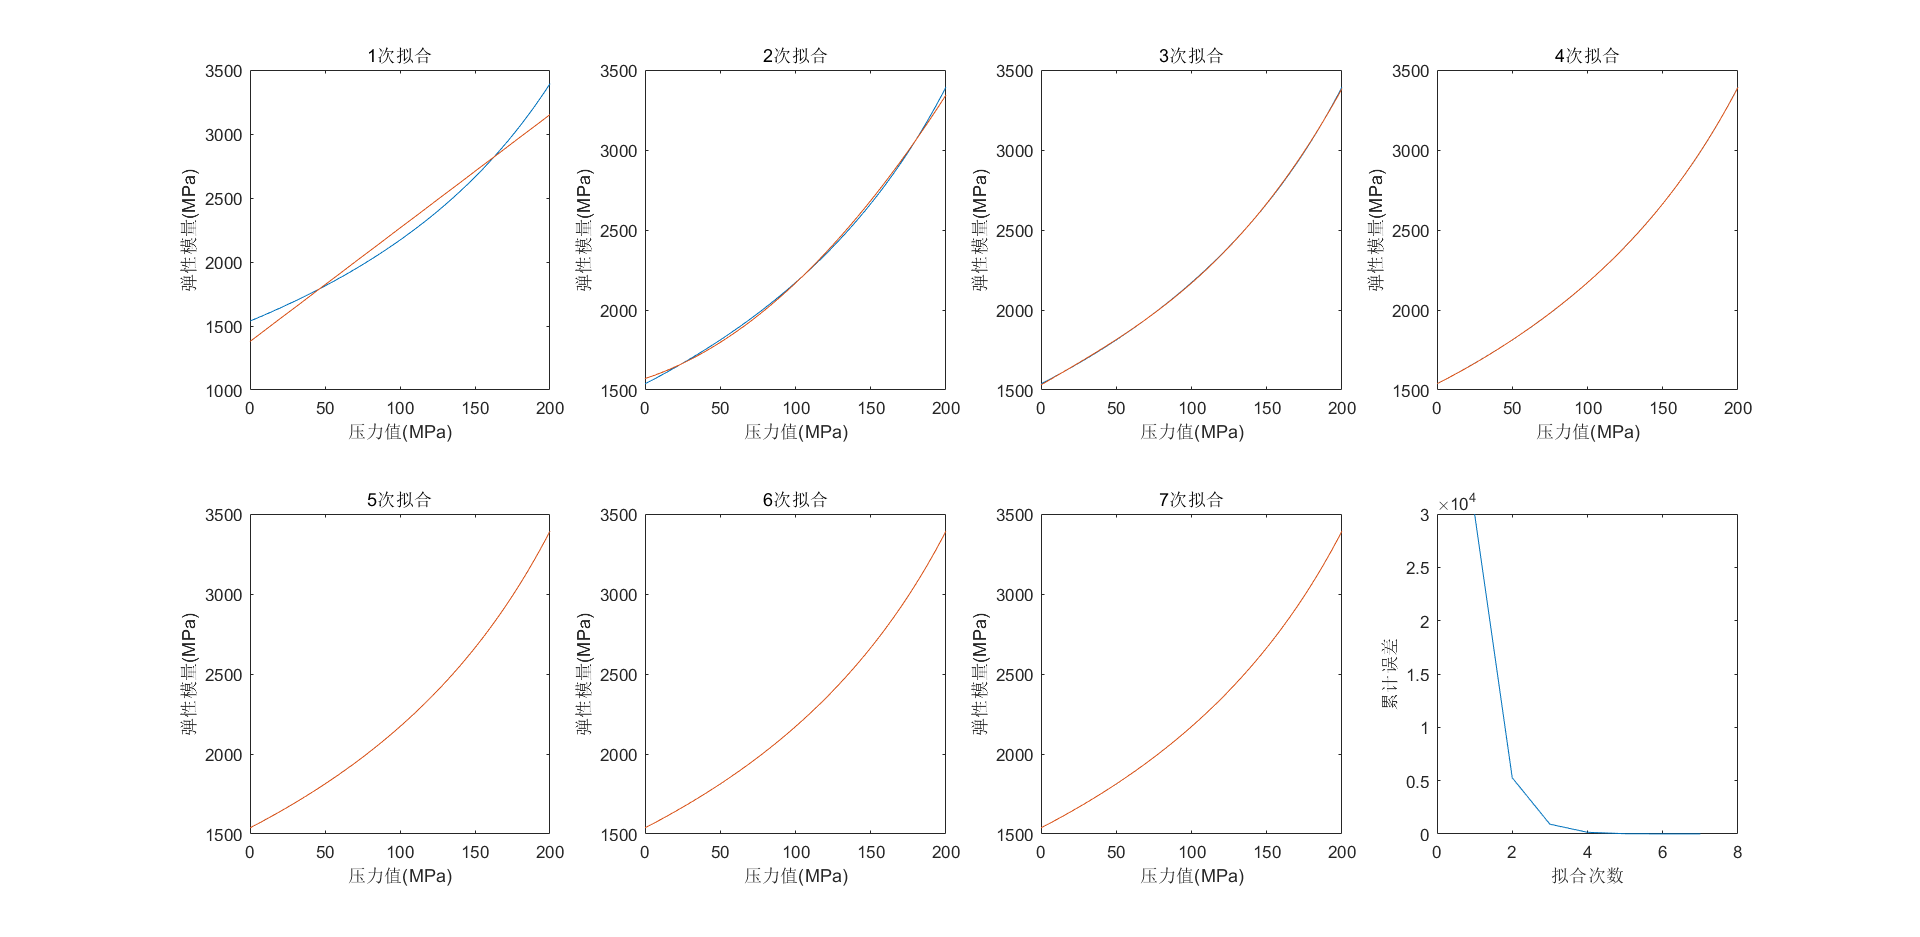
\includegraphics[width=0.9\linewidth]{0-1.png}
	\caption{7次估计的结果及其误差-次数曲线}
	\label{fig:}
\end{figure}

由上图可知,当次数为6次时,其误差已经降低到了较小规模,且梯度急速下降,故本文采用六次函数进行拟合即可,其具体函数如下式:

\begin{equation}
	\begin{aligned}
		E(P)&=1.538\times 10^3+12.140\times P+0.727\times P^2+1.461\times 10^{-4}\times P^3\\
			&+1.172\times 10^{-5}\times P^4-1.2106\times 10^{-7}\times P^5+9.9214\times 10^{-10}\times P^5
	\end{aligned}
\end{equation}

其中,公式系数随着阶数的增大量级迅速减小是因为$P$的数据规模较大(K量级),高次运算会导致量级爆炸。在编程中,会引入较高的误差最终导致系数矩阵的奇异性,严重降低计算精度。故在也运算中首先采用归一化将P的规模缩减为0-1,但是此举在计算的同时也会导致一定的精度丢失(在7次拟合时误差发生反弹的原因)。

故通过以上计算我们定量化了微分方程。但是由于1/E为一个分母多项式函数,其并不一定可积,故采用四阶龙格 -库塔公式进行计算。如下所示:

\begin{equation}
	\left\{
		\begin{array}{ll}
			y_{n+1}=y_n+\frac{h}{6}(K_1+2K_2+2K_3+K_4)\\
			K_1=f(x_n,y_n) \\
			K_2=f(x_n+\frac{h}{2},y_n+\frac{h}{2}K_1)\\
			K_3=f(x_n+\frac{h}{2},y_n+\frac{h}{2}K_2)\\
			K_4=f(x_n+h,y_n+h K_3)
	\end{array} \right.
\end{equation}

令步长分辨为+0.001与-0.001,则可求出$P \in [0,200] \text{MPa} $内所对应的密度。同时采用单步法对过程进行模拟,两者的对比效果如下图所示:

\begin{figure}[htpb]
	\centering
	\begin{subfigure}[htpb]{.45\linewidth}
		\centering
		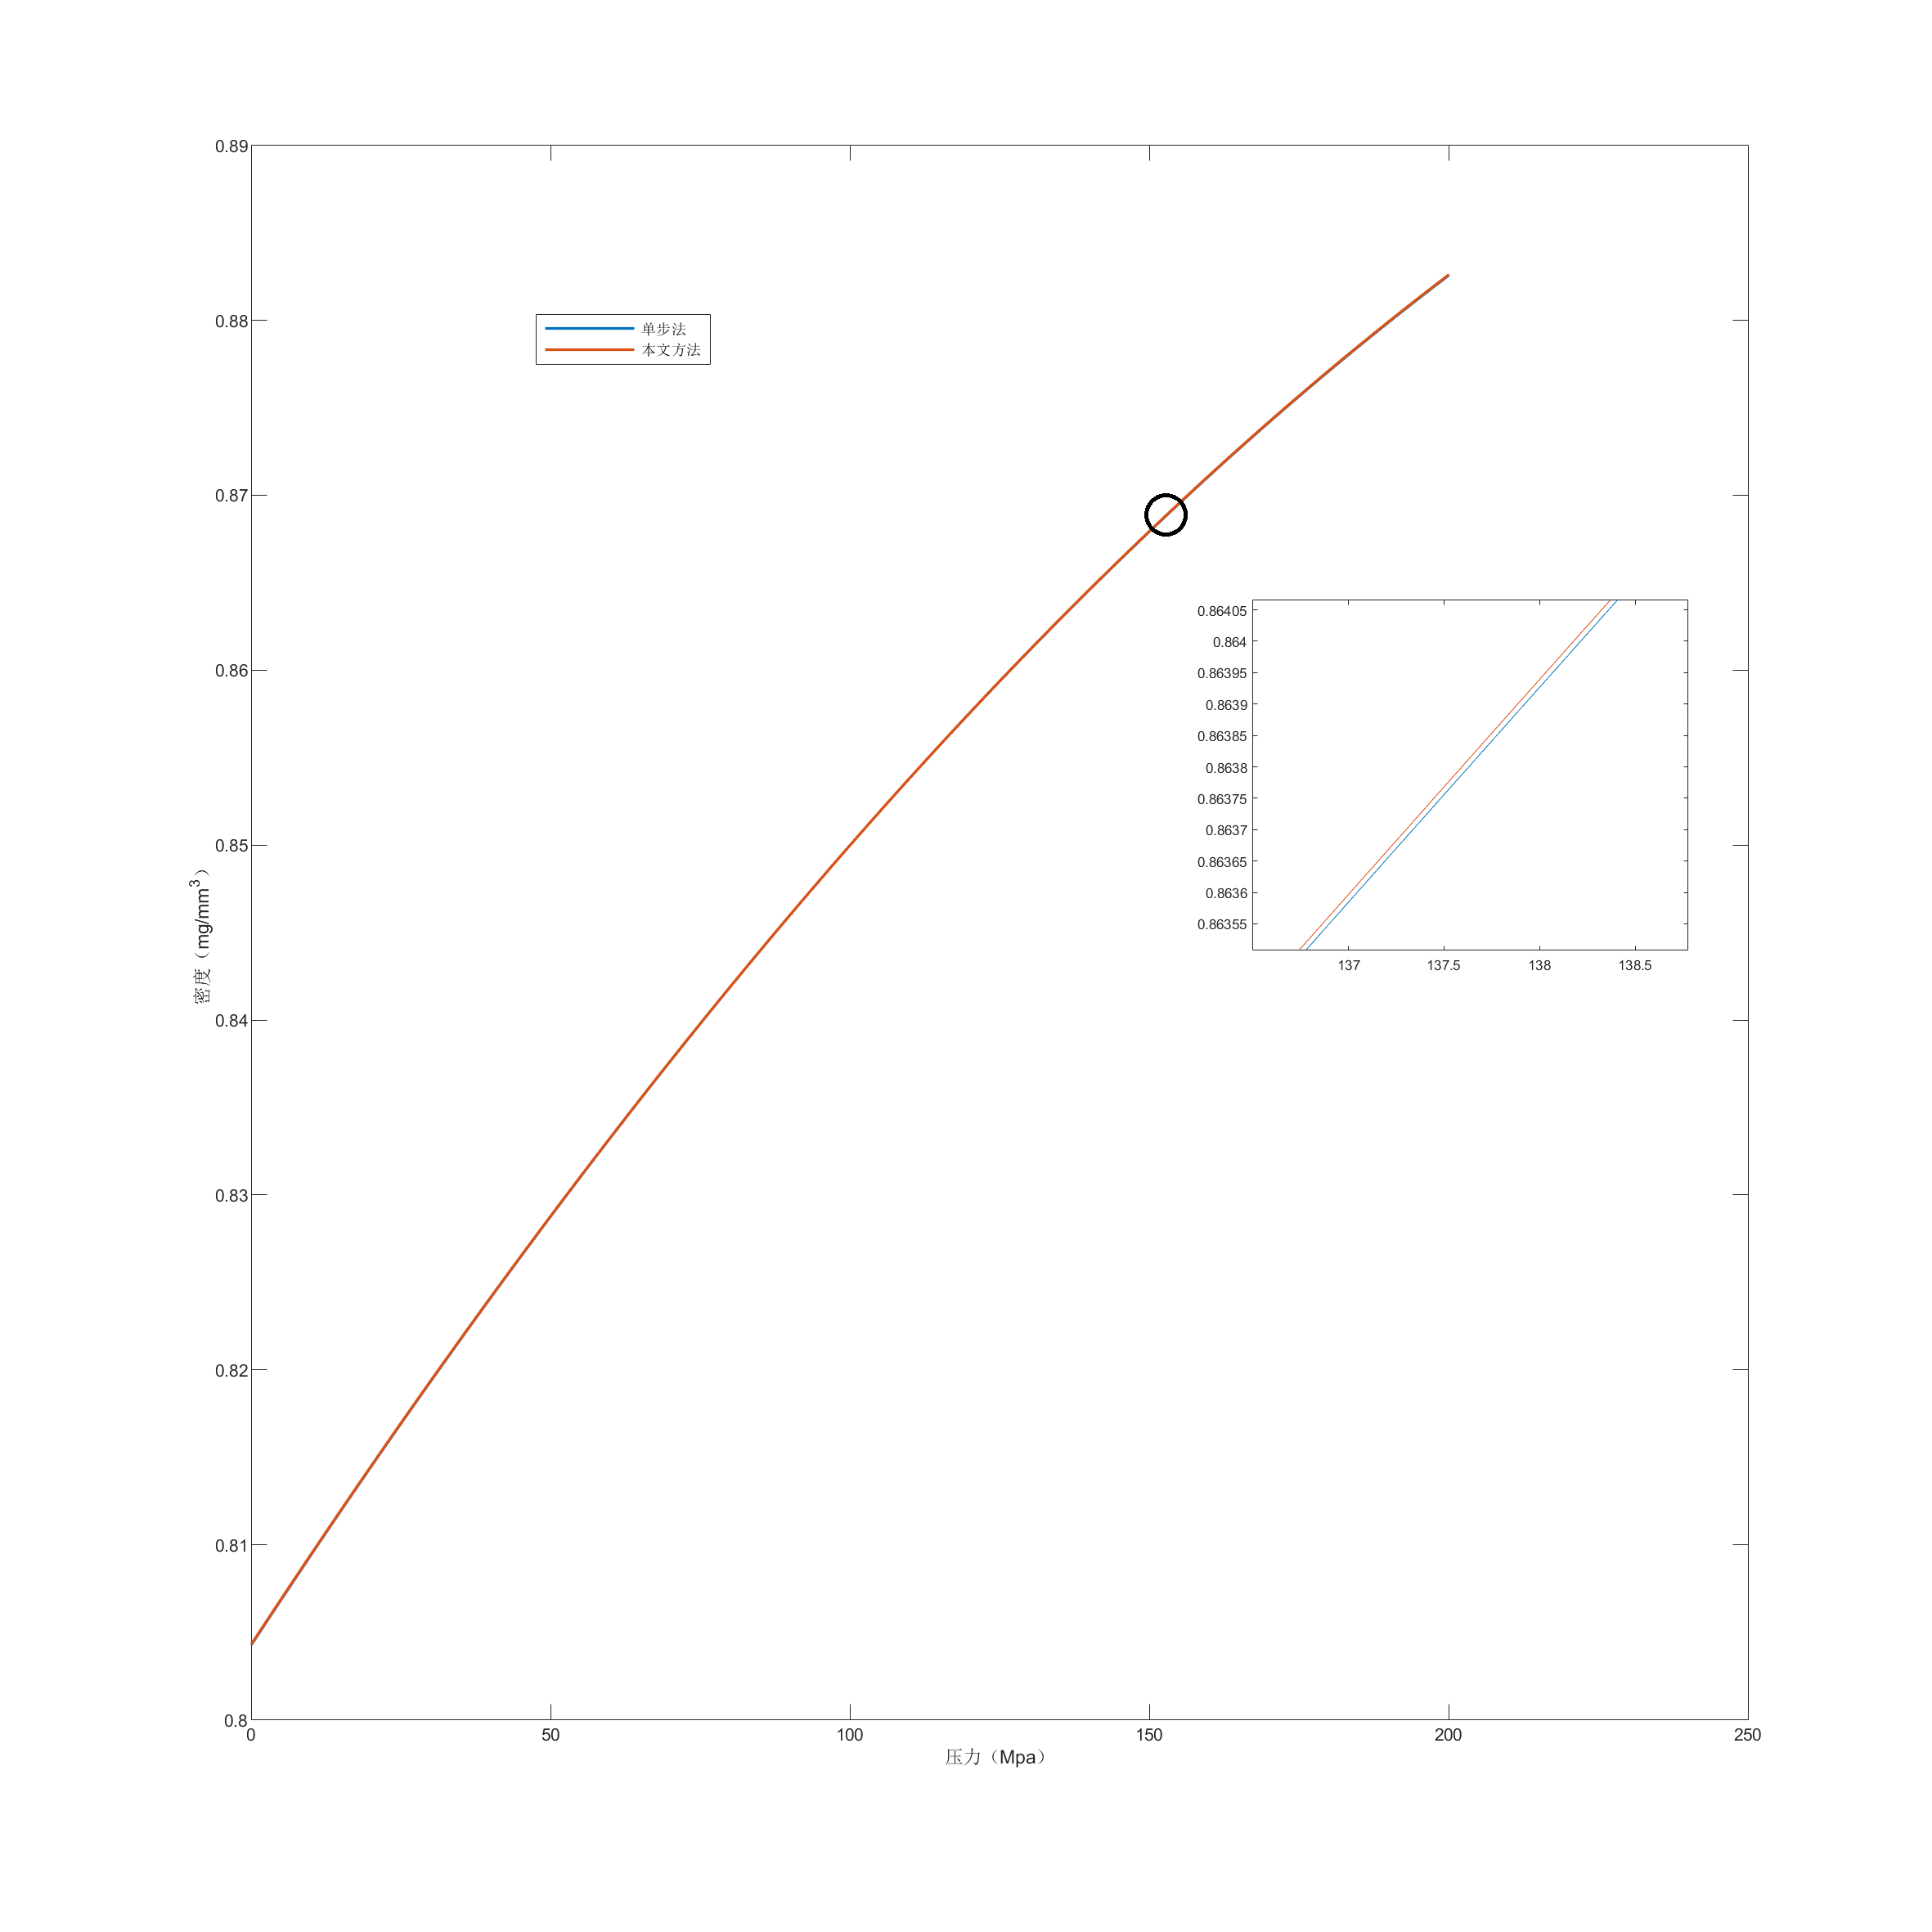
\includegraphics[width=\linewidth]{1-1.png}
		\caption{结果比较}
		\label{fig:结果比较}
	\end{subfigure}
	\quad
	\begin{subfigure}[htpb]{.45\linewidth}

		\centering
		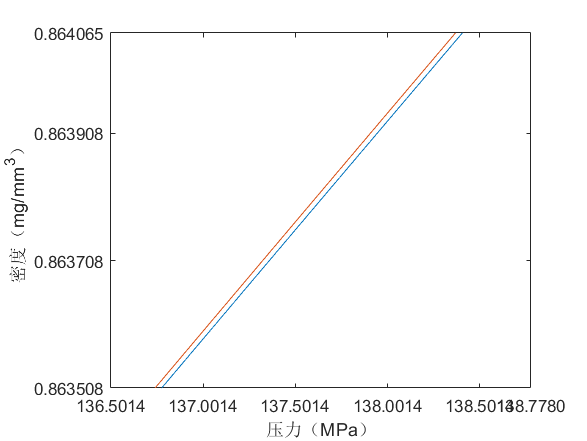
\includegraphics[width=\linewidth]{1-2.png}
		\caption{放大图}
		\label{fig:放大图}
	\end{subfigure}
	\caption{单步法和四阶龙哥库塔法结果比较}
	\label{fig:单步法和四阶龙哥库塔法结果比较}
\end{figure}

从数值上来看,本文方法与传统单步方法相差较少,但是由于动力学系统往往是一个非线性系统\cite{2002计算方法引论},若不进行自保则往往会出现混沌现象,即具有明显的初值稳定性问题。其能达到的精度越高,对于同样预测时长内的数据其可信度与准确的越高。

\subsection{系统仿真实现}
我们采用给定步长$\text{d}t$与步数$n_{\text{step}}$,对系统进行迭代仿真。在每一步内,其高压油泵压力、高压油管压力、高压油泵密度、高压油泵密度等状态参量都近似恒等于该时刻开始时的状态参量。其基本的仿真流程如下图所示:
\begin{figure}[H]
	\centering
	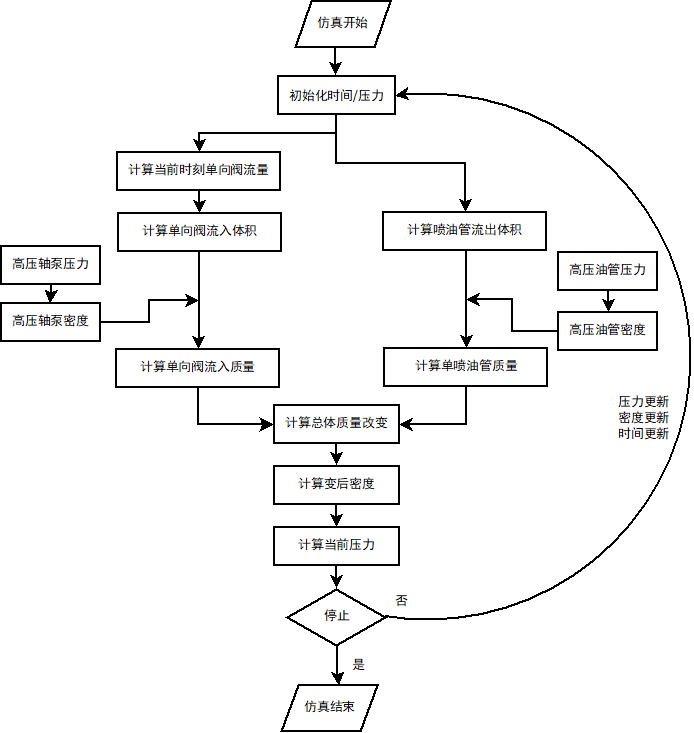
\includegraphics[width=\linewidth]{1-5.png}
	\caption{仿真流程图}
	\label{fig:}
\end{figure}

\section{模型求解}
\subsection{问题一}
根据问题1的描述,高压油管的内腔长度为$500\text{mm}$,内直径为$10\text{mm}$,即可求出高压油管的体积$V_0$为$3.927\times 10^4\text{mm}^3$,供油入口A处小孔的直径为$1.4\text{mm}$,即可求出供油入口的面积$S_A$为$1.5394\text{mm}^2$,通过单向阀供油时间稍微$time_{\text{on}}($\text{ms}$)$,单向阀每打开一次后就要关闭 $10\text{ms}$,即周期为$time_{\text{on}}+10(\text{ms})$。喷油器每秒工作 $10$ 次,即单次工作时长为$100\text{ms}$。每次工作时喷油时间为 $2.4\text{ms}$。

由于喷油过程为一个非恒定的过程,故在仿真过程中需要进行分段处理。而单段时间$[t_0,t_0+\text{d}t]$内位于的区间可能导致一定的计算差异,故我们采用一个分段函数对其进行刻画,其基本情况如下图所示:
\begin{figure}[H]
	\centering
	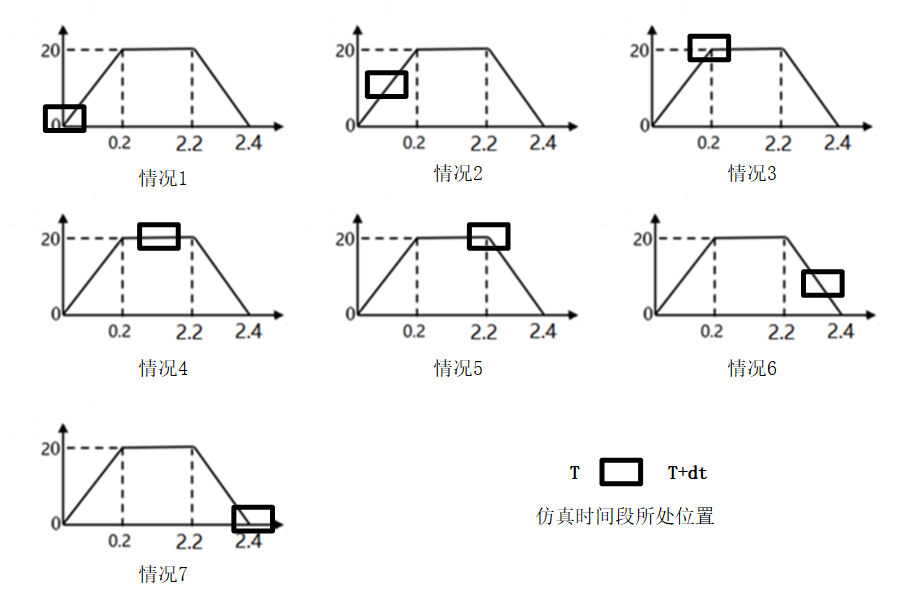
\includegraphics[width=0.7\linewidth]{1-3.png}
	\caption{分段函数}
	\label{fig:}
\end{figure}

由于喷油周期与进油周期并不一致,本文对喷油周期的起始点进行延迟,延迟的范围为$[0,100]\text{ms}$。首先对$time_{\text{on}}\in[0.2,0.4]$包括延迟进行仿真,并对仿真数据与$100\text{Mpa}$进行比较,得到其累计误差,仿真结果如下图所示:
\begin{figure}[H]
	\centering
	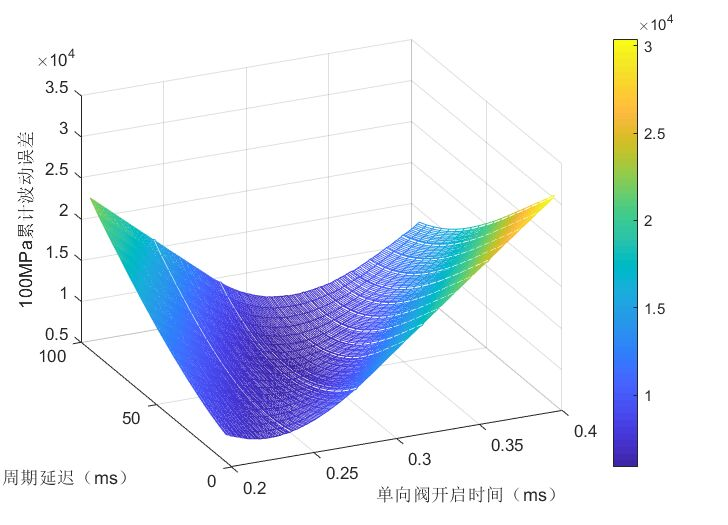
\includegraphics[width=0.7\linewidth]{1-4.png}
	\caption{仿真流程图}
	\label{fig:}
\end{figure}

从仿真结果可以看出,其是一个明显的凸优化过程,而且仅有一个唯一的势能最低点,故本文利用梯度下降法(贪心算法)对其进行求解可得,误差最小的时候,单项阀开启时间为$0.2920\text{ms}$,周期延迟为$60\text{ms}$。

如图\ref{fig:示意图},通过修改单向阀开启时间和周期延迟,可以稳定压强在不同的数值。

\begin{figure}[H]
	\centering
	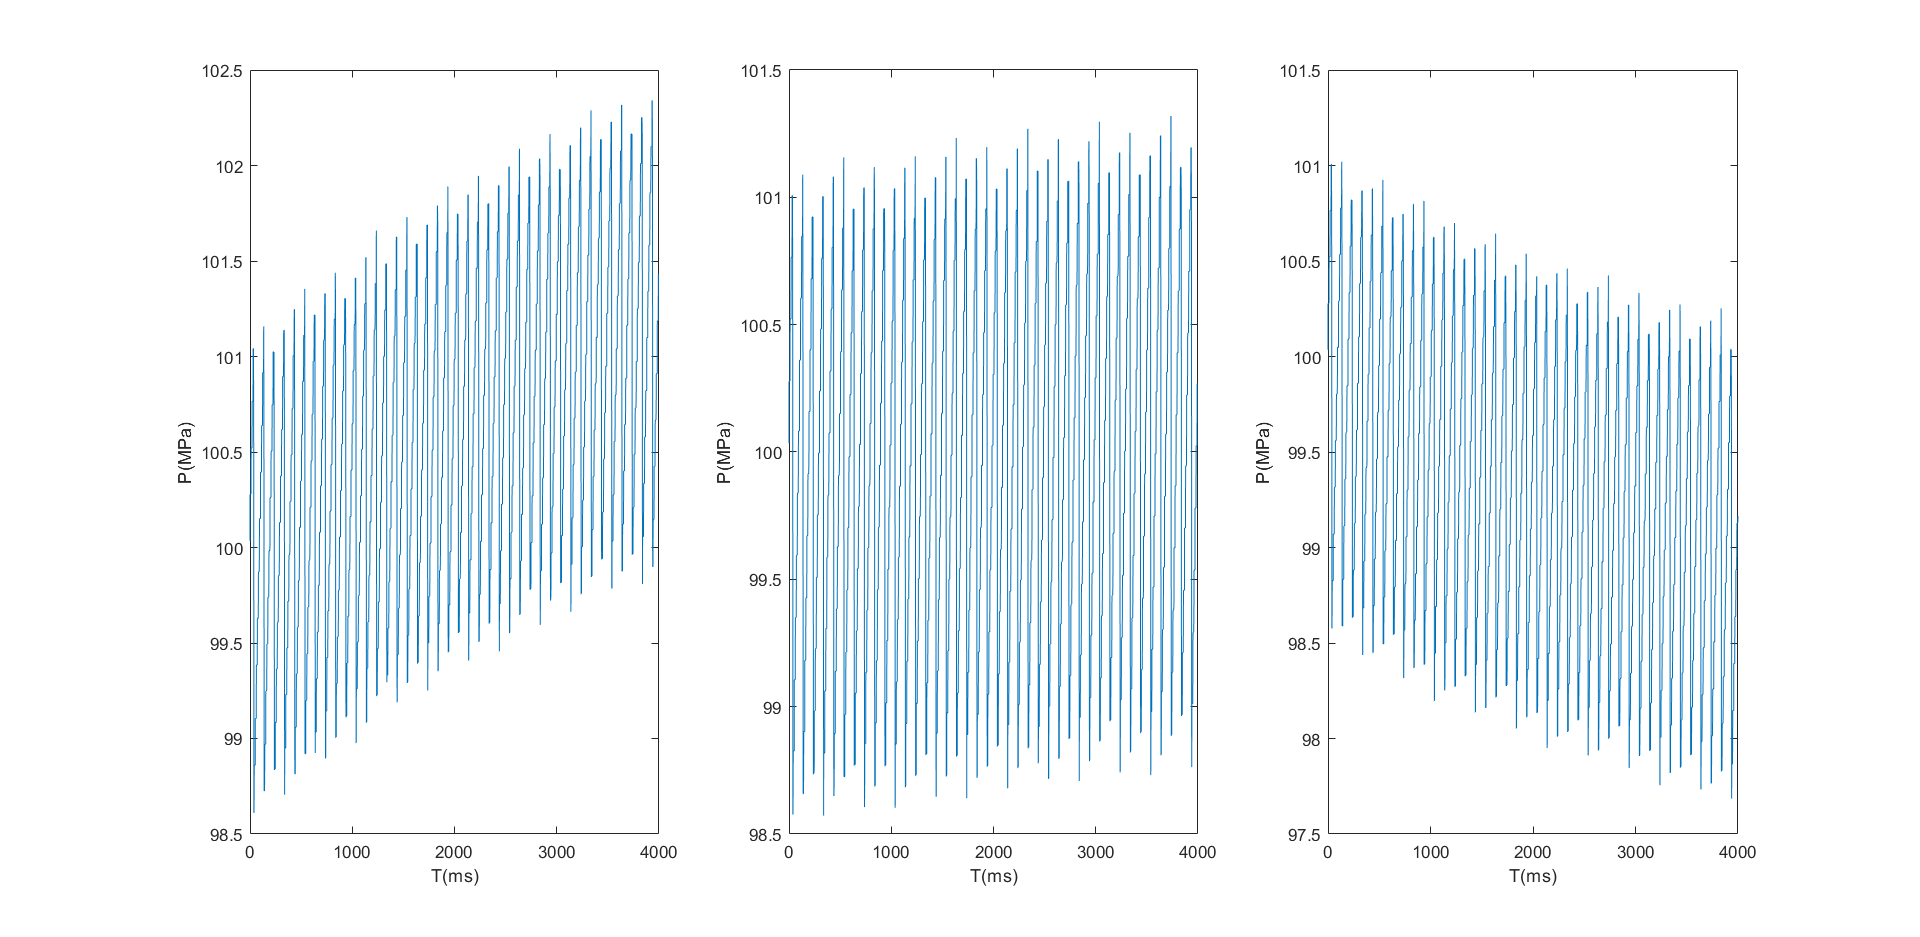
\includegraphics[width=0.8\linewidth]{1-6.png}
	\caption{示意图}
	\label{fig:示意图}
\end{figure}

如图\ref{fig:稳定在100MPa的示意图},压强被稳定在100MPa。

\begin{figure}[H]
	\centering
	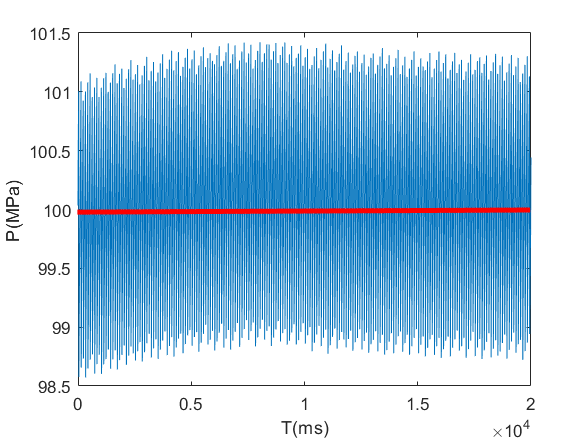
\includegraphics[width=0.6\linewidth]{1-7.png}
	\caption{稳定在100MPa的示意图}
	\label{fig:稳定在100MPa的示意图}
\end{figure}

如图\ref{fig:稳定在150MPa的示意图},压强被稳定在150MPa。

\begin{figure}[H]
	\centering
	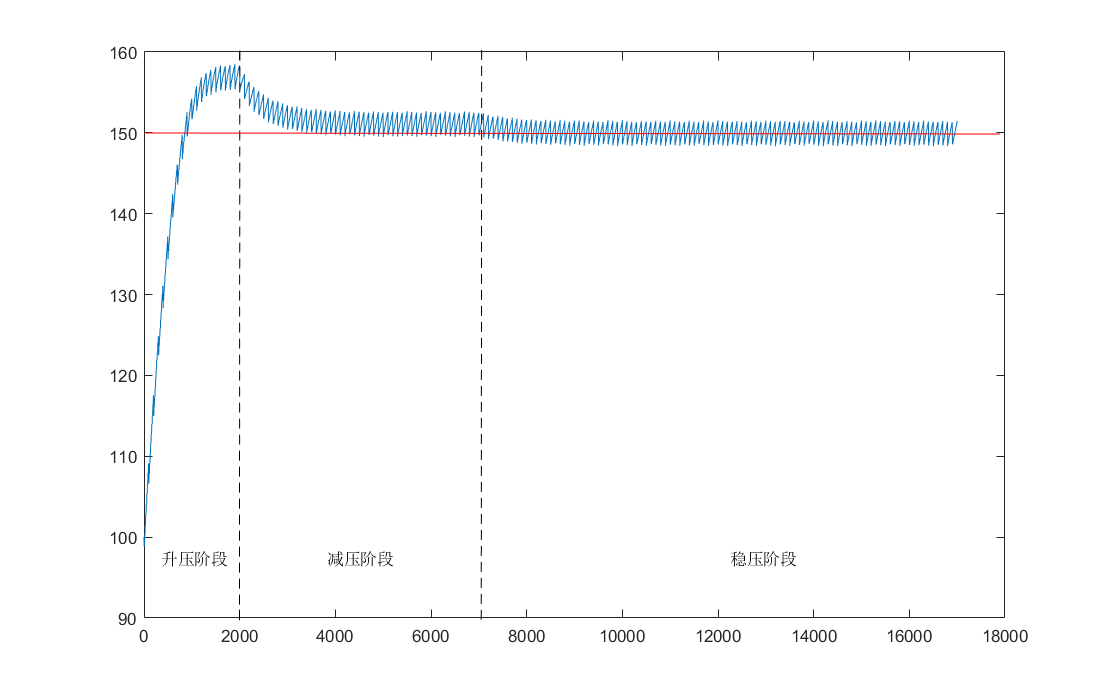
\includegraphics[width=0.6\linewidth]{1-8.png}
	\caption{稳定在150MPa的示意图}
	\label{fig:稳定在150MPa的示意图}
\end{figure}

对于第二问和第三问,只是改变了喷油嘴流量和油泵流量的函数,从原来的随时间的确定性关系变成了随凸轮角速度、减速阀开启时刻、开启时间等的更加复杂的关系。计算量大大增加,在使用Matlab的并行计算和GPU加速的情况下耗时极长。极难求出最优解。故考虑遗传算法,详细说附录\ref{sec:代码}。

第二问是第三问在喷油嘴个数为2,减速阀始终关闭的情况下寻找最优的角速度。属于第三问的特殊情况。

如下图,为考虑凸轮角速度为527弧度每秒,喷油嘴个数为1,减速阀不开的情况下油管压力的曲线。在转过200弧度后稳定在了100.6MPa。

\begin{figure}[H]
	\centering
	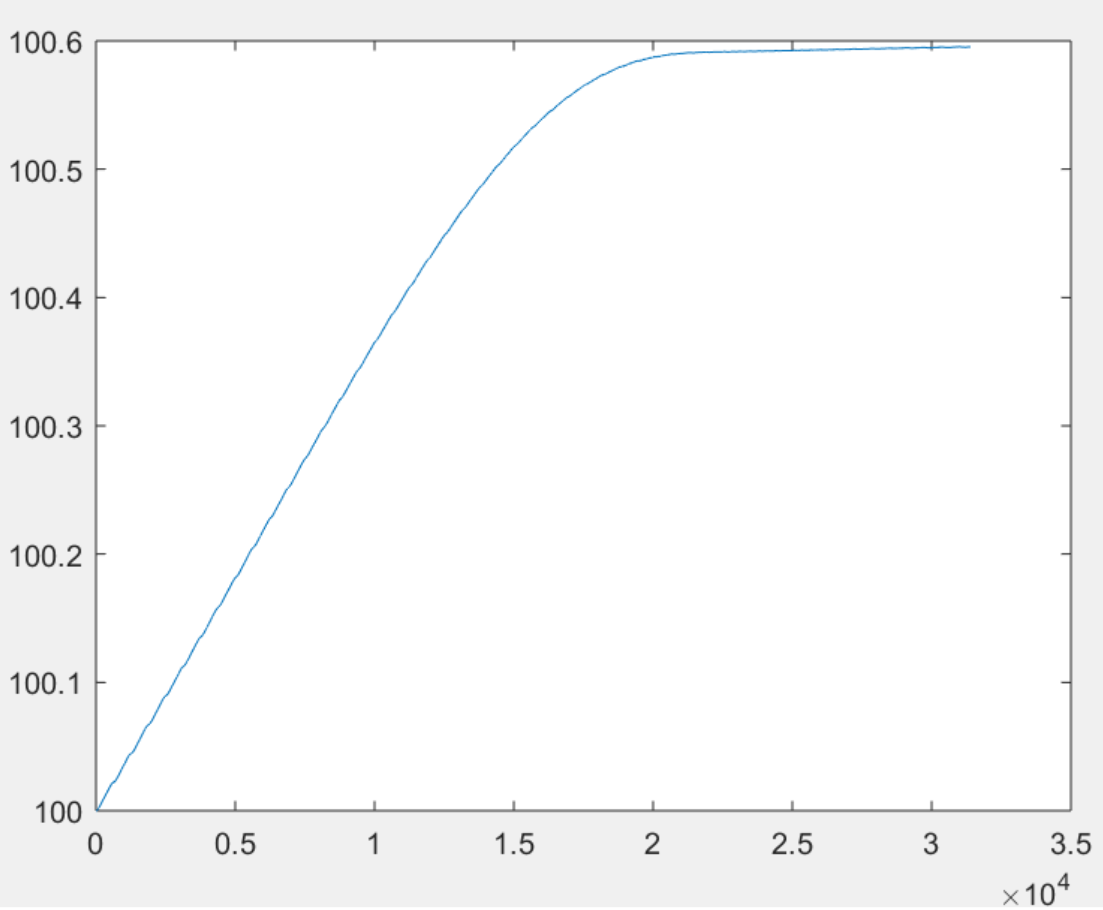
\includegraphics[width=0.5\linewidth]{0.png}
	\caption{问题二}
	\label{fig:问题二}
\end{figure}

如下图,为考虑凸轮角速度为650弧度每秒,喷油嘴个数为2,减速阀开启时间占周期187/628的情况下油管压力的曲线。在转过100弧度后稳定在了96.5MPa。怀疑这是某个非最小值的极值点。但这已经是几次求解中找到的最好结果了。

\begin{figure}[H]
	\centering
	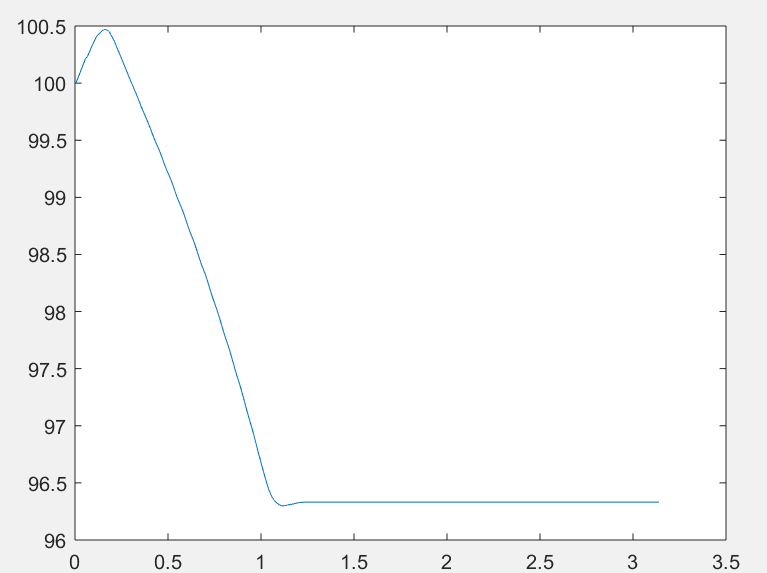
\includegraphics[width=0.5\linewidth]{3.png}
	\caption{问题三}
	\label{fig:问题三}
\end{figure}

\section{评价与改进}%
\label{sec:评价与改进}

\subsection{优点}
\begin{enumerate}
	\item 对喷油过程进行了符合实际、准确的建模,从而求出了较为信服的解。
\end{enumerate}
\subsection{缺点}
\begin{enumerate}
	\item 本文使用的算法在条件更加复杂且时间、计算资源有限的情况下难以得到最优解。
\end{enumerate}

% Fakesection 参考文献

\bibliographystyle{IEEEtran}
\bibliography{src/main}

% Fakesection 附录

\renewcommand{\thesection}{\Alph{section}~}

\appendix

\section{代码}%
\label{sec:代码}

因篇幅所限,只展示了核心代码。附件中的main\_getrho.m通过龙哥库塔法调用Le\_SQ.m 求出压力和密度的关系。核心代码main\_1.m利用压力和密度的关系求出最终结果。其中cal\_Q.m,find\_P.m,find\_rho.m 等子模块求出流量,压强和密度。Prob\_12.m 负责求出压强和密度。

第2问和第3问的main\_2.m和main\_3.m 试图穷举最优解。因条件所限未能如愿。后改用遗传算法main\_GA.m并在化简了许多情况(凸轮匀速转动,减速阀周期变化)后的得到了可能的较优解。原来的main\_2.m 和 main\_3.m 也在附件中一并提交。有兴趣的读者可以试着运行一下看看有多慢。

\langCVfile[Matlab][lst:main.m][Matlab]{main\_1.m}{\string"src/main_1.m\string"}

% Fakesection 索引

\printindex
\end{document}

